\documentclass[]{exam}
\usepackage[utf8]{inputenc}
\usepackage{enumitem}
\usepackage{amsmath}
\usepackage{amsfonts}
\usepackage{setspace}
\usepackage{verbatim} 
\usepackage{graphicx} 
\usepackage{gensymb}
\usepackage{color}
\usepackage{commath}
\usepackage{fancyvrb}
\doublespacing
\graphicspath{{C:\Users\Johnnia\Desktop\常用\Spring2017\CSE 373\HW6}}
\title{}

%===> Formatting ===>
\setlength{\parskip}{8pt}
\setlength{\parindent}{20pt}
%<=== Formatting <===


\title{CSE 373 HW6 Write Up}
\author{Chongyi Xu}

\begin{document}
	
\maketitle
\begin{questions}
\question Using Quick Sort, with the median pivot rule (pick the median of: data[lo], data[hi - 1], and data[(hi + lo) / 2]), sort the following list of numbers. Show your work by drawing the tree of partitions and pivots (as seen in the lecture slides) with the partition rules discussed in lecture (swapping the pivot to index lo and doing swaps to complete the partitions). Apply a cutoff of 3 elements and sort with any sorting method. 
data= [5, 7, 9, 1, 3, 4, 6, 8, 2]
\\
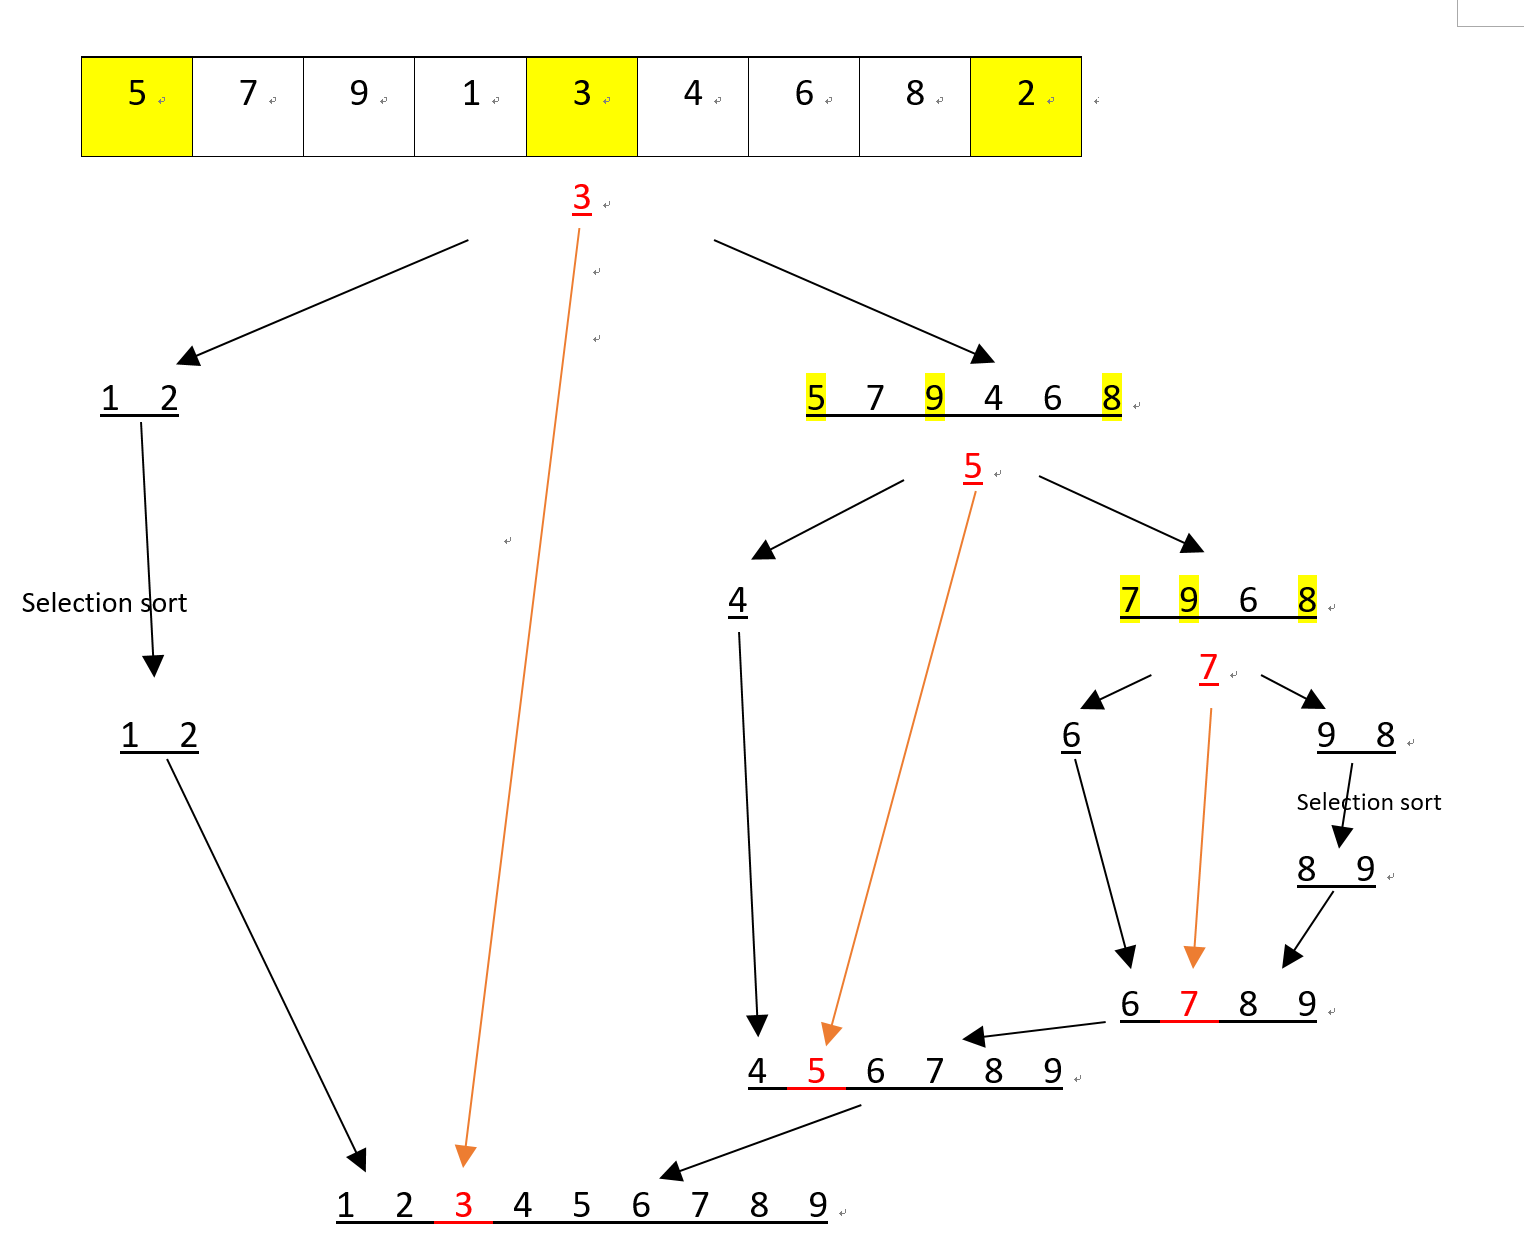
\includegraphics[scale = 0.2]{1.png}

\question Using Radix Sort with a radix of 6 (letters: a, b, c, d, e, f) to alphabetically sort the following strings, draw contents of each bucket at the end of each radix 'digit' iteration pass. 
Strings = (abc, da, ffff, defcd, abebd, ca, b, fef, dfe)
\\
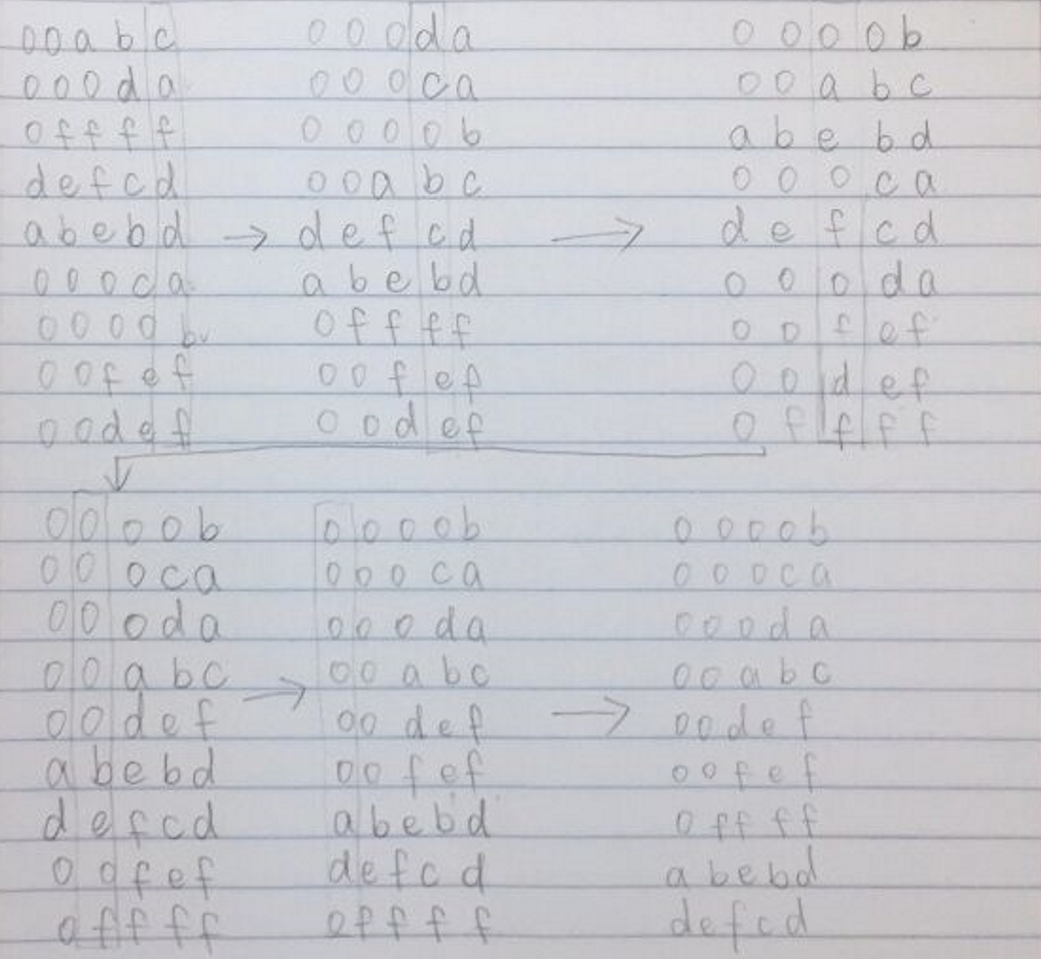
\includegraphics[scale = 0.4]{3.png}
\end{questions}
\end{document}